\documentclass{article}
\usepackage[utf8]{inputenc}
\usepackage{mathpazo} % Palatino font
\usepackage{natbib}
\usepackage{graphicx}
\usepackage{amsmath}
\usepackage{amssymb}
\usepackage{ragged2e}
\usepackage{subfig}

\bibliographystyle{abbrv} %format des citations

\begin{document}
\begin{titlepage}
	\newcommand{\HRule}{\rule{\linewidth}{0.5mm}}
		
	\center
		
	\textsc{\LARGE Université de Bordeaux}\\[1.5cm]
		
	\textsc{\Large Master 1 Informatique}\\[0.5cm]
		
	\textsc{\large Projet de programmation}\\[0.5cm]
		
	\HRule\\[0.4cm]
		
	{\huge\bfseries Cahier d'analyse des besoins}\\[0.4cm]
	\HRule\\[1.5cm]
		
	\begin{minipage}{0.4\textwidth}
		\begin{flushleft}
			\large
			\textit{Auteurs}\\
		    \textsc{Amadou Bah}  Elhajd 
			\\
			\textsc{Deguillaume} Nicolas
			\\
			\textsc{Jolliet} Louis
			\\
			\textsc{Loison} Jules 
			\\
			\textsc{Vigneau} Paul 
		\end{flushleft}
	\end{minipage}
	\vfill\vfill\vfill
		
	{\large 31 Janvier 2019}
	\vfill\vfill
	
\includegraphics[width=0.5\textwidth]{ressources/Logo.jpg}\\[1cm]
		\vfill
		\end{titlepage}
		\justify
		\renewcommand{\contentsname}{Table des matières}
		\tableofcontents
		\newpage
		
		\section{Introduction au projet}
		\paragraph{}
		Notre client souhaite une application qui permet de générer des playlists de titres musicaux selon les goûts d'un groupe composé d'un certain nombre d'utilisateurs en utilisant l'API de Spotify ou Deezer. L'intérêt principal de ce projet est de créer un produit qui puisse être utilisé par des chercheurs du LaBRI, leur permettant de tester différents algorithmes. En effet l'application doit proposer un ou plusieurs algorithmes ayant pour but de générer des playlists composées de musiques plaisant le plus possible à tous les utilisateurs. Pour ce faire, l'application doit récupérer les informations d'écoute de ces utilisateurs (musiques appréciées, playlists personnelles, genres les plus écoutés, etc). 
		    
		Ensuite, l'application doit permettre à l'utilisateur d'écouter cette playlist nouvellement générée, en embarquant un lecteur de musique comprenant des options basiques telles que changer de musique, faire pause, reprendre, mettre un "j'aime", etc. L'application doit pouvoir récupérer les logs d'écoute (chaque interaction avec le lecteur) afin de pouvoir analyser et évaluer les différents algorithmes. Une fois l'application produite, les chercheurs du LaBRI pourront ensuite ajouter et analyser de nouveaux algorithmes plus complexes, mais nous devons néanmoins en implémenter. 
		    
		Enfin, des points importants soulignés par le client, destinés à nous guider au moment de prendre certains choix d'implémentation, sont que le produit doit être assez intuitif, rapide et simple d'utilisation. 
		
		Nous avons choisi d'utiliser l'API de Spotify afin de réaliser l'application car nous sommes plus familiers avec ce service.     
		\section{Description et analyse de l'existant}
		\paragraph{}
		Nous démarrons notre application de zéro, cependant il existe certains exemples nous permettant d'avoir des idées de fonctionnalités ou de design. Pour le moment, les seuls exemples dont nous pouvons nous inspirer qui correspondent le plus à ce que nous devons réaliser sont Friends Mix par Apple et Family Mix par Spotify. En effet, Apple Music propose un mix, renouvelé chaque semaine incluant les 25 chansons les plus écoutées par nos amis. De la même façon, Spotify, dans leur offre Premium Family (pouvoir avoir jusqu'à 6 utilisateurs sur un même compte), offre une playlist incluant les goûts de chacun. Ces applications possèdent un certain nombre des fonctionnalités énoncées en \ref{besoins}, il est bien sûr impossible de customiser l'algorithme de génération des playlist, ce qui est le but premier de notre client. Nous pouvons cependant nous inspirer certaines fonctionnalités disponibles et pouvons améliorer l'expérience utilisateur, tel que la provenance des musiques (de quel(s) utilisateur(s) provient la musique) comme on peut le voir sur la Figure \ref{fig:example}.
		
		
		De plus nous allons nous servir de différents dépots GitHub utilisant les API Spotify \cite{spotify-web-api} ou Deezer.
		
        \begin{figure}%
            \centering
            \subfloat[Freinds Mix - Apple Music]{{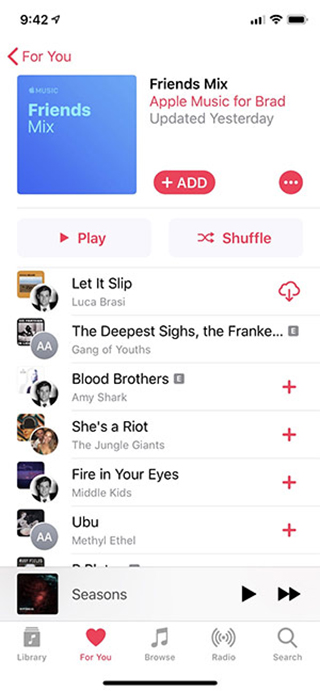
\includegraphics[width=5cm]{ressources/friends-mix-apple-music.jpg} }}%
            \qquad
            \subfloat[Family Mix - Spotify]{{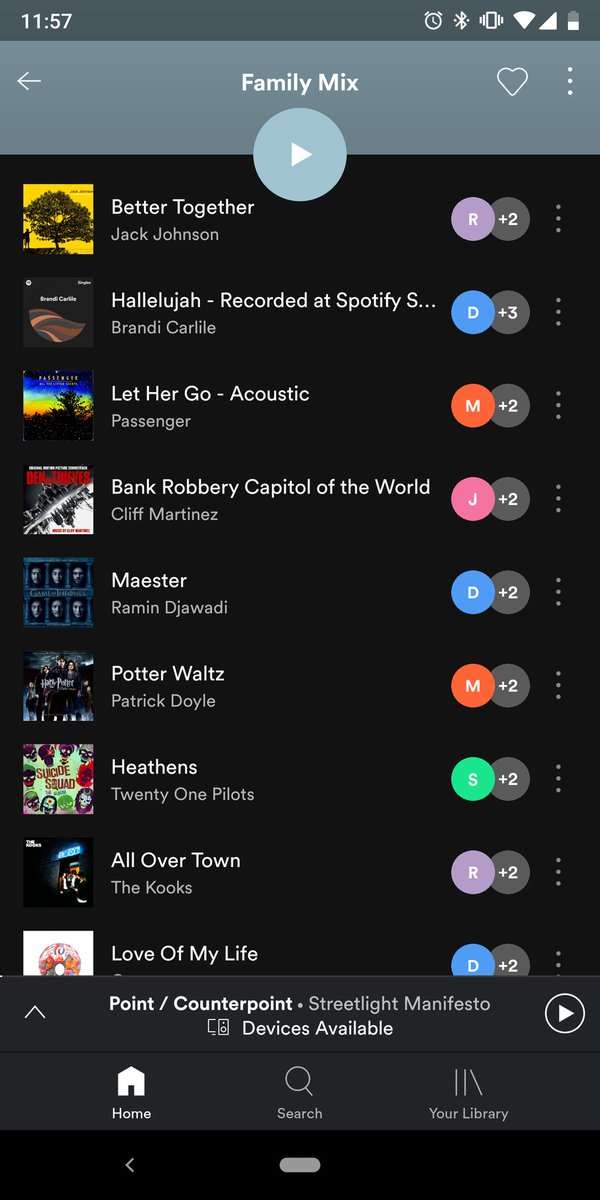
\includegraphics[width=5cm]{ressources/Spotify_Family_Mix.jpg} }}%
            \caption{Exemple d'applications similaires}%
            \label{fig:example}%
        \end{figure}

		\section{Description des besoins} \label{besoins}
		Afin de décrire la priorité de chaque besoin, nous écrirons au début de la description d'un besoin un de ces mots :
		\begin{itemize}
			\item \textbf{Essentiel} : le logiciel ne sera pas acceptable sans que ce besoin soit réalisé
			\item \textbf{Conditionnel} : besoin qui étend et améliore le logiciel, sans que ce besoin soit nécessaire pour rendre le logiciel acceptable
			\item \textbf{Optionnel} : besoin dont la valeur n’est pas encore assurée. Donne au fournisseur l’occasion de proposer quelque chose qui va au-delà des besoins attendus
		\end{itemize}
		\subsection{Besoins fonctionnels}
		Nous détaillerons les besoins suivants, exprimés par le client :
		\subsubsection{Connexion de plusieurs utilisateurs} \label{connexion}
		\textbf{[ Essentiel ]}
		\begin{itemize}
			\item L'utilisateur principal doit pouvoir lancer une nouvelle session
			\item Il se connecte via une pop-up d'authentification sur Spotify pour que les requêtes fonctionnent 
			\item Tous les autres utilisateurs peuvent se rechercher comme sur Spotify s'il suivent l'utilisateur principal en utilisant le même appareil
			\item Les utilisateurs peuvent ensuite s'ajouter à la session
			\item L'utilisateur principal doit pouvoir se déconnecter, ce qui aura pour effet de supprimer la session
		\end{itemize}
		\textbf{[ Conditionnel ]}
		\begin{itemize}
			\item Un utilisateur doit pouvoir être ignoré dans l'algorithme (fonction "mute")
			\item Un utilisateur doit pouvoir être retiré du groupe
		\end{itemize}
		
		\subsubsection{Accès aux informations de chaque utilisateur} 
		Une fois un utilisateur ajouté (cf. \ref{connexion}), il faut donc accéder à ses chansons préférées via l'API choisie. 
		\\
		\textbf{[ Essentiel ]}
		\begin{itemize}
			\item Récupérer les informations des utilisateurs, nécessaires au fonctionnement des algorithmes de génération de playlists, grâce à l'API Spotify (playlists publiques)
		\end{itemize}
		\textbf{[ Conditionnel ]}
		\begin{itemize}
			\item Récupérer d'autres informations comme les chansons aimées ou artistes préférés
		\end{itemize}
		\subsubsection{Proposition de playlist(s)}
		\textbf{[ Essentiel ]}
	      \begin{itemize}
	        \item L'utilisateur doit pouvoir lancer un mix (ce qui aura pour effet de lancer l'algorithme)
	      	\item L'application devra pouvoir créer une playlist vide
	      	\item Et ajouter des titres à cette playlist locale
	      \end{itemize}
  	    \textbf{[ Optionnel ]}
        \begin{itemize}
      	    \item Pouvoir ajouter les playlists au compte Spotify de l'utilisateur principal
        \end{itemize}
        Les playlists peuvent contenir jusqu'à 10 000 titres néanmoins nous ne les générerons qu'avec 25 titre pour commencer. Le chiffre pourra éventuellement grandir dans le futur en fonction des performances de notre application et des algorithmes utilisés. (cf. \ref{performance})
			        

		\subsubsection{Proposer différents algorithmes de génération de playlists}
	    \textbf{[ Essentiel ]}
		\begin{itemize}
			\item  L'application proposera au moins un algorithme \cite{ICDM2017} permettant de tester les fonctionnalités proposées par le produit final
			\item Il sera possible de changer d'algorithme dans les options
		\end{itemize}
	    \textbf{[ Conditionnel ]}
		\begin{itemize}
			\item  L'application proposera d'autres algorithmes \cite{ICDM2017} plus complexes permettant une réelle analyse des données
		\end{itemize}
		  
		\subsubsection{Lecture de ces playlists, avec possibilité de skipper des titres}
		\paragraph{}
		L'application utilisera le WEB Player SDK qui permet, entre autres, les mêmes interactions avec la musique que le lecteur de l'application officielle. Afin d'utiliser le WEB Player SDK, l'utilisateur principal devra disposer d'un compte premium. Les utilisateurs pourront donc effectuer les interactions suivantes: \newline \newline
		\textbf{[ Essentiel ]}
		\begin{itemize}
			\item play/pause
			\item skip/back
			\item like
		\end{itemize}
		\subsubsection{Récupération des logs d'écoute pour évaluation des algorithmes} \label{logs}
		\textbf{[ Essentiel ]}
		\begin{itemize}
	    			\item Ce besoin peut se découper en plusieurs sous-besoins :
			      \begin{itemize}
			      	\item Récupérer les méta-données de la session d'écoute grâce au WEB Player SDK
			      	\item Créer un fichier JSON sur l'appareil de l'utilisateur
			      	\item Y renseigner les méta-données précédemment obtenues
			      \end{itemize}
	    \end{itemize}
	    \textbf{[ Optionnel ]}
		\begin{itemize}
        \item Envoie du fichier par email pour simplifier l'analyse
		\end{itemize}
		\subsubsection{Faire fonctionner l'application avec l'API de Deezer}
	    \textbf{[ Optionnel ]}
		\begin{itemize}
		    \item Les algorithmes resteront les mêmes néanmoins il faudra dupliquer et adapter tout ce qui utilise l'API Spotify pour que cela fonctionne avec l'API Deezer. On peut imaginer une fenêtre à l'ouverture de l'application qui demande si l'utilisateur souhaite utiliser Deezer ou Spotify
		\end{itemize}
		\subsection{Besoins non fonctionnels}
		  \subsubsection{Performance} \label{performance}
		  \textbf{[ Essentiel ]}
		  \begin{itemize}
		      \item L'application doit être rapide pour générer des playlists. Une playlist générée s'affichera et se lancera dès l'algorithme terminé (à la façon de la fonctionnalité "shuffle play" sur Spotify). Les utilisateurs doivent attendre au maximum quelques secondes avant de pouvoir lancer une musique
		  \end{itemize}
		    \subsubsection{Accord d'utilisation de données}
		    \textbf{[ Essentiel ]}
		    \begin{itemize}
		    \item L'application s'ouvrira affichant les conditions d'utilisation. Il sera alors demandé aux utilisateurs leur accord pour collecter les logs d'utilisation de l'application, optionnellement (cf. \ref{logs}), les transmettre au client automatiquement et utiliser les identifiants Spotify renseignés pour récupérer les informations nécessaires à la génération de playlist
		   \end{itemize}
		   \subsubsection{Ergonomie}
		   \textbf{[ Essentiel ]}
		   \begin{itemize}
		   \item L'utilisateur doit pouvoir comprendre comment utiliser l'application au premier coup d'oeil et répondre à des standards d'ergonomie (densité des éléments, disposition, couleurs...)
		   \item Il doit lui être rapide d'écouter de la musique sur l'application.
		   \item Des pistes d'interface sont (seront) disponibles dans le partie \ref{prototype}
		   \end{itemize}
		\subsection{Scénarios, prototypes, schémas et diagrammes UML} \label{prototype}
		\section{Gantt}
		\section{Bibliographie}
		\bibliography{references}
		
\end{document} 